


\noindent 
\textbf{\stepcounter{zadatak}
\thecjelina.\thezadatak.}
Vanjska sila $F_0$ djeluje na blok A mase $m_A= 5\ kg$ koji vuče blok B mase $m_B= 3\ kg$ (vidjeti skicu). Nerastezljiva nit kojom su blokovi spojeni može podnjeti silu napetosti od  $T=21\ N$, a zatim puca. Izračunajte maksimalni iznos sile $F_0$ kojom možemo vući blok A. Koeficijent kinetičkog trenja između blokova i podloge je $\mu_k=0.4$.


\begin{figure}[h]%{r}{0.7\textwidth} % Inline image example
  \begin{center}
    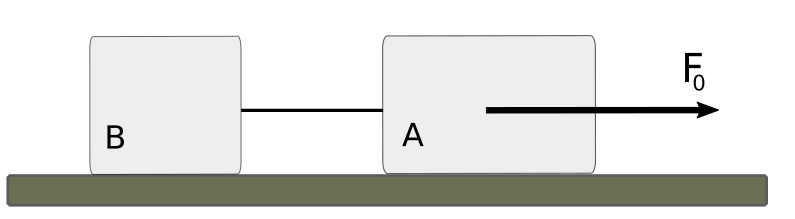
\includegraphics[scale=0.30]{../03_Dinamika_materijalne_tocke/Zadatak_D301.png}
  \end{center}
  %\caption{Fish}
\end{figure}


